\documentclass{article}
\usepackage{amsmath, sfmath, multicol, tkz-euclide, array, enumerate, tcolorbox, tabularray}
\renewcommand{\familydefault}{\sfdefault}
\setlength{\parindent}{0cm}
\pagestyle{empty}
\usepackage[left=1in, top=0.5in, right=1in, bottom=0.5in]{geometry}
\tikzset{>=stealth}
\tcbset{colback=white}

\newcounter{example}[section]
\newenvironment{example}[1][]{\refstepcounter{example}\par\medskip
   {\color{red}\textbf{Example~\theexample. #1}}}{\medskip}

\begin{document}

\section*{Triangle Congruence by ASA and AAS}

\begin{tcolorbox}[colframe=orange!70!white, coltitle=black, title=\textbf{Today I Can}]
\begin{enumerate}
    \item Prove triangles congruent by ASA and SAS shortcuts.
\end{enumerate}
\end{tcolorbox}

\begin{tcolorbox}[colframe=black!20!white, opacitybacktitle=0.1, coltitle=black, title=\textbf{Angle-Side-Angle (ASA) Shortcut}]
If 2 angles and the included side of one triangle are congruent to 2 angles and the included side of another triangle, then the triangles are congruent.
\newline

\begin{minipage}{0.3\textwidth}
\begin{itemize}
    \item $\triangle ABC \cong \triangle DEF$
\end{itemize}
\end{minipage}
\begin{minipage}{0.6\textwidth}
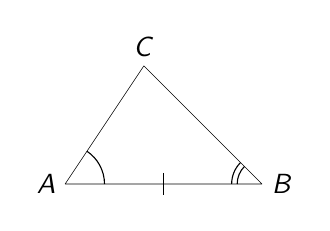
\begin{tikzpicture}
\tkzDefPoints{0/0/A, 2.5/0/B, 1/1.5/C}
\tkzDrawPolygon(A,B,C)
\tkzLabelPoints[right](B)
\tkzLabelPoints[left](A)
\tkzLabelPoints[above](C)
\tkzMarkAngle[size=0.5](B,A,C)
\tkzMarkAngle[arc=ll, size=0.35](C,B,A)
\tkzMarkSegment[mark=|](A,B)
\end{tikzpicture}
\hspace{0.25in}
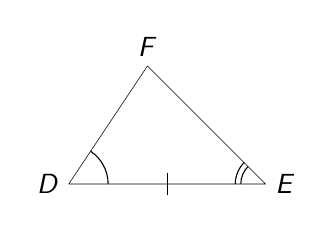
\begin{tikzpicture}
\tkzDefPoints{0/0/A, 2.5/0/B, 1/1.5/C}
\tkzDrawPolygon(A,B,C)
\tkzLabelPoint[right](B){$E$}
\tkzLabelPoint[left](A){$D$}
\tkzLabelPoint[above](C){$F$}
\tkzMarkAngle[size=0.5](B,A,C)
\tkzMarkAngle[arc=ll, size=0.35](C,B,A)
\tkzMarkSegment[mark=|](A,B)
\end{tikzpicture}
\end{minipage}
\end{tcolorbox}

\bigskip 

\begin{example}
Which two triangles are congruent by ASA? Explain.
\begin{enumerate}[(a)]
    \item \mbox{} \newline 
    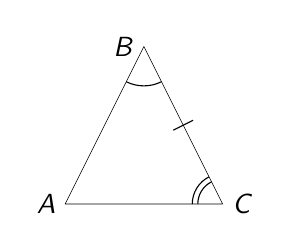
\begin{tikzpicture}
    \tkzDefPoints{0/0/A, 2/0/C, 1/2/B}
    \tkzDrawPolygon(A,B,C)
    \tkzLabelPoint[left](A){$A$}
    \tkzLabelPoint[left](B){$B$}
    \tkzLabelPoint[right](C){$C$}
    \tkzMarkSegment[mark=|](B,C)
    \tkzMarkAngle[size=0.5](A,B,C)
    \tkzMarkAngle[arc=ll, size=0.35](B,C,A)
\end{tikzpicture}
\hspace{0.2in}
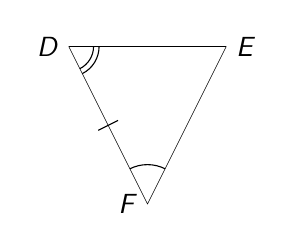
\begin{tikzpicture}
    \tkzDefPoints{0/0/A, -2/0/C, -1/-2/B}
    \tkzDrawPolygon(A,B,C)
    \tkzLabelPoint[right](A){$E$}
    \tkzLabelPoint[left](B){$F$}
    \tkzLabelPoint[left](C){$D$}
    \tkzMarkSegment[mark=|](B,C)
    \tkzMarkAngle[size=0.5](A,B,C)
    \tkzMarkAngle[arc=ll, size=0.35](B,C,A)
\end{tikzpicture}
\hspace{0.2in}
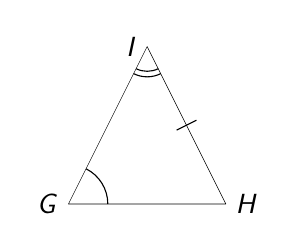
\begin{tikzpicture}
    \tkzDefPoints{0/0/A, 2/0/C, 1/2/B}
    \tkzDrawPolygon(A,B,C)
    \tkzLabelPoint[left](A){$G$}
    \tkzLabelPoint[left](B){$I$}
    \tkzLabelPoint[right](C){$H$}
    \tkzMarkSegment[mark=|](B,C)
    \tkzMarkAngle[size=0.5](C,A,B)
    \tkzMarkAngle[arc=ll, size=0.35](A,B,C)
\end{tikzpicture}
\vspace{0.5in} 
    \item \mbox{} \newline 
    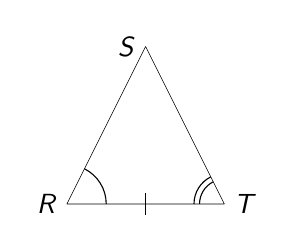
\begin{tikzpicture}
    \tkzDefPoints{0/0/A, 2/0/C, 1/2/B}
    \tkzDrawPolygon(A,B,C)
    \tkzLabelPoint[left](A){$R$}
    \tkzLabelPoint[left](B){$S$}
    \tkzLabelPoint[right](C){$T$}
    \tkzMarkSegment[mark=|](A,C)
    \tkzMarkAngle[size=0.5](C,A,B)
    \tkzMarkAngle[arc=ll, size=0.35](B,C,A)
\end{tikzpicture}
\hspace{0.2in}
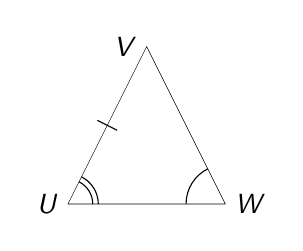
\begin{tikzpicture}
    \tkzDefPoints{0/0/A, 2/0/C, 1/2/B}
    \tkzDrawPolygon(A,B,C)
    \tkzLabelPoint[left](A){$U$}
    \tkzLabelPoint[left](B){$V$}
    \tkzLabelPoint[right](C){$W$}
    \tkzMarkSegment[mark=|](A,B)
    \tkzMarkAngle[size=0.5](B,C,A)
    \tkzMarkAngle[arc=ll, size=0.35](C,A,B)
\end{tikzpicture}
\hspace{0.2in}
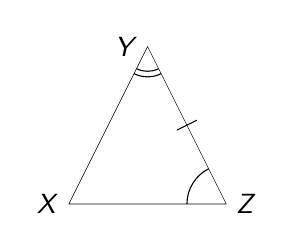
\begin{tikzpicture}
    \tkzDefPoints{0/0/A, 2/0/C, 1/2/B}
    \tkzDrawPolygon(A,B,C)
    \tkzLabelPoint[left](A){$X$}
    \tkzLabelPoint[left](B){$Y$}
    \tkzLabelPoint[right](C){$Z$}
    \tkzMarkSegment[mark=|](B,C)
    \tkzMarkAngle[size=0.5](B,C,A)
    \tkzMarkAngle[arc=ll, size=0.35](A,B,C)
\end{tikzpicture}
\end{enumerate}
\end{example}

\vspace{0.5in}

\begin{example}
\textbf{Given:} $\angle CAB \cong \angle DAE$, $\overline{BA} \cong \overline{EA}$, $\angle B$ and $\angle E$ are right angles.    \quad
\textbf{Prove:} $\triangle ABC \cong \triangle AED$
\newline\\

\begin{tikzpicture}
    \tkzDefPoints{0/0/B, 2/0/A, 4/0/E, 0/2.5/C, 4/2.5/D}
    \tkzDrawPolygon(B,E,D,A,C)
    \tkzLabelPoints[below](B,A,E)
    \tkzLabelPoints[left](C)
    \tkzLabelPoints[right](D)
\end{tikzpicture}
\end{example}

\vfill 
\newpage 

\begin{tcolorbox}[colframe=black!20!white, opacitybacktitle=0.1, coltitle=black, title=\textbf{Angle-Angle-Side (AAS) Shortcut}]
If 2 angles and a non-included side of one triangle are congruent to 2 angles and a non-included side of another triangle, then the triangles are congruent.
\newline

\begin{minipage}{0.3\textwidth}
\begin{itemize}
    \item $\triangle ABC \cong \triangle DEF$
\end{itemize}
\end{minipage}
\begin{minipage}{0.6\textwidth}
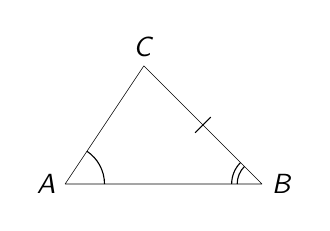
\begin{tikzpicture}
\tkzDefPoints{0/0/A, 2.5/0/B, 1/1.5/C}
\tkzDrawPolygon(A,B,C)
\tkzLabelPoints[right](B)
\tkzLabelPoints[left](A)
\tkzLabelPoints[above](C)
\tkzMarkAngle[size=0.5](B,A,C)
\tkzMarkAngle[arc=ll, size=0.35](C,B,A)
\tkzMarkSegment[mark=|](C,B)
\end{tikzpicture}
\hspace{0.25in}
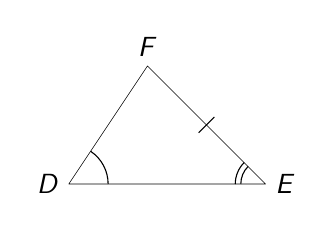
\begin{tikzpicture}
\tkzDefPoints{0/0/A, 2.5/0/B, 1/1.5/C}
\tkzDrawPolygon(A,B,C)
\tkzLabelPoint[right](B){$E$}
\tkzLabelPoint[left](A){$D$}
\tkzLabelPoint[above](C){$F$}
\tkzMarkAngle[size=0.5](B,A,C)
\tkzMarkAngle[arc=ll, size=0.35](C,B,A)
\tkzMarkSegment[mark=|](C,B)
\end{tikzpicture}
\end{minipage}
\end{tcolorbox}

\bigskip 

\begin{example}
Prove each of the following. 
\begin{enumerate}[(a)]
    \item \textbf{Given:} $\angle M \cong \angle K$, $\overline{WM} \parallel \overline{RK}$ \quad 
 \textbf{Prove:} $\triangle WMR \cong \triangle RKW$ \newline\\ 
    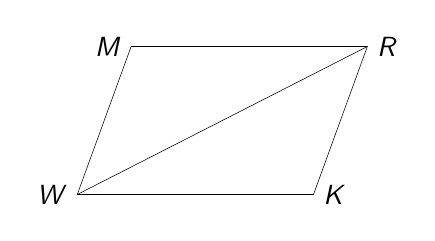
\begin{tikzpicture}
    \tkzDefPoints{0/0/W, 3/0/K}
    \tkzDefShiftPoint[W](70:2){M}
    \tkzDefShiftPoint[K](70:2){R}
    \tkzDrawPolygon(W,K,R,M)
    \tkzDrawSegment(W,R)
    \tkzLabelPoints[left](W,M)
    \tkzLabelPoints[right](R,K)
\end{tikzpicture}
\vfill 
    \item \textbf{Given:} $\angle S \cong \angle Q$, $\overline{RP}$ bisects $\angle SRQ$ \quad  \textbf{Prove:} $\triangle SRP \cong \triangle QRP$ \newline\\
    \begin{tikzpicture}
    \tkzDefPoints{0/0/R, 0/3.5/P}
    \tkzDefShiftPoint[R](40:2){Q}
    \tkzDefShiftPoint[R](140:2){S}
    \tkzDrawPolygon(R,S,P,Q)
    \tkzDrawSegment(R,P)
    \tkzLabelPoints[below](R)
    \tkzLabelPoints[left](S)
    \tkzLabelPoints[above](P)
    \tkzLabelPoints[right](Q)
\end{tikzpicture}
\end{enumerate}
\end{example}
\vfill 

\begin{example}
Are $\triangle PAR$ and $\triangle SIR$ congruent? Explain.
\newline\\

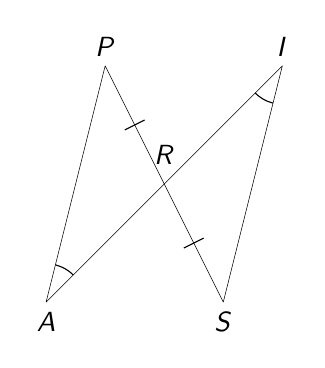
\begin{tikzpicture}[scale=0.75]
    \tkzDefPoints{0/0/A, 1/4/P, 4/4/I, 3/0/S, 2/2/R}
    \tkzDrawPolygon(A,P,S,I)
    \tkzLabelPoints[below](A,S)
    \tkzLabelPoints[above](I,P)
    \tkzLabelPoints[above, yshift=0.05in](R)
    \tkzMarkAngles[size=0.65](R,A,P R,I,S)
    \tkzMarkSegments[mark=|](P,R S,R)
\end{tikzpicture}
\end{example}

\end{document}
